%% METADATA
%% subject-code: DI01000061
%% subject-name: Modern Physics
%% semester: 1
%% examination: Summer-2025
%% date: 11-06-2025
%% description: Solution guide for Modern Physics
%% tags: study-material, solutions, gtu, DI01000061
%% END METADATA

\documentclass{article}

% content/resources/templates/preamble.tex
\usepackage[margin=0.6in]{geometry}
\author{Milav Dabgar}
\usepackage{amsmath,amssymb,amsthm}
\usepackage{booktabs}
\usepackage{multirow}
\usepackage{xcolor}
\usepackage{tcolorbox}
\tcbuselibrary{breakable,skins}
\usepackage[colorlinks=true,linkcolor=blue]{hyperref}
\usepackage{titlesec}
\usepackage{enumitem}
\usepackage{tikz}
\usepackage{pgfplots}
\usepackage{circuitikz}
\usepackage[version=4]{mhchem}
\usepackage{longtable}
\usepackage{array}
\usepackage{float}
\usepackage{caption}
\usepackage{listings}

\lstset{
  basicstyle=\small\ttfamily,
  breaklines=true,
  breakatwhitespace=false,
  postbreak=\mbox{\textcolor{red}{$\hookrightarrow$}\space},
  float=false,
  numbers=left,
  numberstyle=\tiny\color{gray},
  numbersep=10pt,
  xleftmargin=2em,
  keywordstyle=\color{blue},
  commentstyle=\color{green!60!black},
  stringstyle=\color{purple},
  backgroundcolor=\color{gray!5},
  showstringspaces=false,
  tabsize=2,
  captionpos=b,
  keepspaces=true,
  columns=flexible
}

\pgfplotsset{compat=1.18}
\usetikzlibrary{shapes,arrows,positioning,calc,patterns,decorations.pathmorphing,decorations.markings,arrows.meta}

% Color scheme
\definecolor{headcolor}{RGB}{0,102,204}
\definecolor{keycolor}{RGB}{220,20,60}
\definecolor{solutioncolor}{RGB}{34,139,34}
\definecolor{mnemoniccolor}{RGB}{148,0,211}
\definecolor{codecolor}{RGB}{0,0,100}

% Spacing
\setlength{\parskip}{3pt}
\setlist[itemize]{nosep}
\setlist[enumerate]{nosep}

% Title formatting
\titleformat{\section}{\Large\bfseries\color{headcolor}}{\thesection}{1em}{}
\titleformat{\subsection}{\large\bfseries\color{headcolor}}{\thesubsection}{1em}{}

% Pandoc tightlist compatibility
\providecommand{\tightlist}{%
  \setlength{\itemsep}{0pt}\setlength{\parskip}{0pt}}

% Pandoc longtable compatibility
\newcounter{none}
\def\thenone{}


\title{Modern Physics (DI01000061) - Summer 2025 Solution}
\date{June 11, 2025}

\hypersetup{
  pdftitle={Modern Physics (DI01000061) - Summer 2025 Solution},
  pdfsubject={GTU Exam Solution - Summer-2025},
  pdfauthor={Milav Dabgar},
  pdfkeywords={study-material, solutions, gtu, DI01000061},
  pdfcreator={xelatex}
}

\begin{document}
\maketitle

\setcounter{tocdepth}{5}
\tableofcontents
\newpage

% ========================================
% QUESTION 1: MCQs (14 marks)
% Demonstrates: 14 single mark questions
% ========================================

\section{Question 1}

\subsection{Question 1(a) [14 marks]}
\textbf{Fill in the blanks/MCQs using appropriate choice from the given options.}

\subsubsection{Solution}

\begin{enumerate}
    \item \textbf{The SI unit of temperature is \_\_\_\_\_\_\_\_\_\_.}
    \begin{enumerate}
        \item Kelvin
        \item Fahrenheit
        \item Celsius
        \item None of these
    \end{enumerate}
    \textbf{Answer:} (1) Kelvin
    \paragraph{Explanation:} The SI (International System of Units) unit of temperature is Kelvin (K). Celsius and Fahrenheit are other scales but not the SI unit.
    \subparagraph{Note:} Absolute zero is 0 K.
    \paragraph{Mnemonic:} \emph{Kelvin is King of SI units.}

    \item \textbf{Coulomb is the SI unit of \_\_\_\_\_\_\_\_\_\_.}
    \begin{enumerate}
        \item electric current
        \item electric potential
        \item electric charge
        \item electric field
    \end{enumerate}
    \textbf{Answer:} (3) electric charge
    \paragraph{Explanation:} The Coulomb (C) is defined as the unit of electric charge, equal to the quantity of electricity conveyed in one second by a current of one ampere.
    \paragraph{Mnemonic:} \emph{C for Charge, C for Coulomb.}

    \item \textbf{0.0031 has \_\_\_\_\_\_\_\_\_\_ significant digits.}
    \begin{enumerate}
        \item 5
        \item 4
        \item 2
        \item 3
    \end{enumerate}
    \textbf{Answer:} (3) 2
    \paragraph{Explanation:} Leading zeros are never significant. Therefore, in 0.0031, only the digits 3 and 1 are significant.
    \paragraph{Mnemonic:} \emph{Leading zeros lose value.}

    \item \textbf{Which type of impurity is added to make P-type semiconductor?}
    \begin{enumerate}
        \item Trivalent
        \item Tetravalent
        \item Pentavalent
        \item None of these
    \end{enumerate}
    \textbf{Answer:} (1) Trivalent
    \paragraph{Explanation:} Trivalent impurities (like Boron, Aluminum) have 3 valence electrons, creating ``holes'' (Positive charge carriers) in the semiconductor lattice, hence P-type.
    \paragraph{Mnemonic:} \emph{P for P-type, P comes after T? No. Trivalent starts with T, Three valence electrons.}

    \item \textbf{Which of the following is non-mechanical wave?}
    \begin{enumerate}
        \item sound wave
        \item light wave
        \item water wave
        \item Ultrasonic wave
    \end{enumerate}
    \textbf{Answer:} (2) light wave
    \paragraph{Explanation:} Light waves are electromagnetic waves and do not require a material medium for propagation, making them non-mechanical. Sound, water, and ultrasonic waves need a medium.
    \paragraph{Mnemonic:} \emph{Light travels through vacuum, so it's non-mechanical.}

    \item \textbf{The quantization of electric charge is represented by\_\_\_\_\_\_\_\_\_\_.}
    \begin{enumerate}
        \item \(Q=ne\)
        \item \(Q=n/e\)
        \item \(Q=e\)
        \item None of these
    \end{enumerate}
    \textbf{Answer:} (1) \(Q=ne\)
    \paragraph{Explanation:} Charge quantization means charge exists in discrete packets. Total charge \(Q\) is an integer multiple \(n\) of the fundamental charge \(e\) (\(1.6 \times 10^{-19} C\)).
    \paragraph{Mnemonic:} \emph{Q = ne (Quarter Needs Energy? No, Quantity = Number * electron).}

    \item \textbf{Frequency range of Infrasonic waves are\_\_\_\_\_\_\_\_\_\_.}
    \begin{enumerate}
        \item Greater than 20KHz
        \item Greater than 10KHz
        \item Between 20Hz to 20KHz
        \item Less than 20Hz
    \end{enumerate}
    \textbf{Answer:} (4) Less than 20Hz
    \paragraph{Explanation:} Infrasonic waves have frequencies below the audible range (less than 20 Hz). Audible is 20 Hz to 20 kHz. Ultrasonic is above 20 kHz.
    \paragraph{Mnemonic:} \emph{Infra means Below (20 Hz).}

    \item \textbf{Snell's law relates\_\_\_\_\_\_\_\_\_\_.}
    \begin{enumerate}
        \item Light transmission
        \item Light diffraction
        \item Light reflection
        \item Light refraction
    \end{enumerate}
    \textbf{Answer:} (4) Light refraction
    \paragraph{Explanation:} Snell's law describes the relationship between the angles of incidence and refraction when light passes between two different isotropic media.
    \paragraph{Mnemonic:} \emph{Snell spells Refraction cells.}

    \item \textbf{Optical fiber operates on the principle of \_\_\_\_\_\_\_\_\_\_ of light.}
    \begin{enumerate}
        \item Polarisation
        \item Refraction
        \item Reflection
        \item Total internal reflection
    \end{enumerate}
    \textbf{Answer:} (4) Total internal reflection
    \paragraph{Explanation:} Optical fibers work by confining light within the core using total internal reflection (TIR), allowing it to travel long distances with minimal loss.
    \paragraph{Mnemonic:} \emph{Fiber traps light totally inside.}

    \item \textbf{Laser radiation is\_\_\_\_\_\_\_\_\_\_.}
    \begin{enumerate}
        \item Monochromatic
        \item Unidirectional
        \item Highly coherent
        \item All of these
    \end{enumerate}
    \textbf{Answer:} (4) All of these
    \paragraph{Explanation:} LASER (Light Amplification by Stimulated Emission of Radiation) is characterized by being monochromatic (single color), unidirectional (low divergence), and coherent (in phase).
    \paragraph{Mnemonic:} \emph{Laser is Perfect Light: one color, one direction, one phase.}

    \item \textbf{In optical fiber cable, the inner part is called\_\_\_\_\_\_\_\_\_\_.}
    \begin{enumerate}
        \item Sheath
        \item Cladding
        \item Core
        \item None of these
    \end{enumerate}
    \textbf{Answer:} (3) Core
    \paragraph{Explanation:} The core is the central part of the optical fiber where light transmission takes place. It is surrounded by cladding which has a lower refractive index.
    \paragraph{Mnemonic:} \emph{Core is the Center.}

    \item \textbf{Which of following is semiconductor material?}
    \begin{enumerate}
        \item Aluminium
        \item Silicon
        \item Gallium
        \item Arsenic
    \end{enumerate}
    \textbf{Answer:} (2) Silicon
    \paragraph{Explanation:} Silicon (Si) and Germanium (Ge) are the most common intrinsic semiconductor materials. Aluminium is a conductor. Gallium and Arsenic are used in compound semiconductors (GaAs).
    \paragraph{Mnemonic:} \emph{Silicon Valley is Semiconductor Valley.}

    \item \textbf{With increase voltage of the forward bias to a PN junction, the width of depletion layer \_\_\_\_\_\_\_\_\_\_.}
    \begin{enumerate}
        \item No change
        \item Increase
        \item Decrease
        \item None of these
    \end{enumerate}
    \textbf{Answer:} (3) Decrease
    \paragraph{Explanation:} In forward bias, the external electric field opposes the potential barrier, pushing majority carriers towards the junction, which reduces (decreases) the width of the depletion layer.
    \paragraph{Mnemonic:} \emph{Forward pushes narrower.}

    \item \textbf{LEDs emit light due to the phenomenon of\_\_\_\_\_\_\_\_\_\_.}
    \begin{enumerate}
        \item Electromagnetic Induction
        \item Electrostatic Discharge
        \item Electroluminescence
        \item Thermal Emission
    \end{enumerate}
    \textbf{Answer:} (3) Electroluminescence
    \paragraph{Explanation:} Electroluminescence is an optical phenomenon and electrical phenomenon in which a material emits light in response to the passage of an electric current.
    \paragraph{Mnemonic:} \emph{Electron to Luminesce (Light).}
\end{enumerate}

% ========================================
% QUESTION 2: Short Questions (14 marks)
% Demonstrates: 3 marks and 4 marks questions
% ========================================

\section{Question 2}

\noindent \textbf{Question 2(a) [6 marks]} \\
\textbf{Answer the following questions. (Any 2 out of 3)}

\subsection{Question 2(a)(1) [3 marks]}
\textbf{Draw neat sketch of micrometre screw gauge and write names of different parts.}

\subsubsection{Solution}
A micrometre screw gauge is a precision instrument used to measure small distances with high accuracy.

\begin{figure}[H]
    \centering
    \includegraphics[width=0.6\linewidth]{micrometer_sketch.png}
    \caption{Micrometer Screw Gauge}\label{fig:micrometer}
\end{figure}

\paragraph{Parts of Micrometre Screw Gauge:}
\begin{itemize}
    \item \textbf{Frame:} It is a U-shaped metallic frame that holds the other parts together. It provides rigidity to the instrument.
    \item \textbf{Anvil:} It is a small fixed stud at one end of the frame against which the object is held.
    \item \textbf{Spindle:} It is a movable cylindrical part that moves towards the anvil when the thimble is rotated.
    \item \textbf{Sleeve (Main Scale):} It is a stationary cylinder with a linear scale marked in millimeters (mm).
    \item \textbf{Thimble (Circular Scale):} It is accurate rotatable part that moves over the sleeve. It carries the circular scale divisions (usually 50 or 100).
    \item \textbf{Ratchet:} It is used to apply uniform pressure on the object. It produces a `click' sound when the spindle touches the object, preventing overtightening.
\end{itemize}

\paragraph{Mnemonic:} \emph{FAST Ratchet (Frame, Anvil, Spindle, Thimble, Ratchet).}

\subsection{Question 2(a)(2) [3 marks]}
\textbf{Explain Coulomb's law with mathematical formula.}

\subsubsection{Solution}
\textbf{Coulomb's Law} states that the magnitude of the electrostatic force of attraction or repulsion between two point charges is directly proportional to the product of the magnitudes of charges and inversely proportional to the square of the distance between them. The force acts along the line joining the two charges.

\paragraph{Mathematical Formula:}
\[ F = k \frac{|q_1 q_2|}{r^2} \]
where:
\begin{itemize}
    \item \(F\) = Electrostatic Force (Newton)
    \item \(q_1, q_2\) = Magnitudes of charges (Coulomb)
    \item \(r\) = Distance between charges (meter)
    \item \(k\) = Coulomb's constant (\(\approx 9 \times 10^9 \, N \cdot m^2 / C^2\))
\end{itemize}
\[ k = \frac{1}{4\pi\epsilon_0} \]
where \(\epsilon_0\) is permittivity of free space.

\paragraph{Mnemonic:} \emph{Force depends on Product of charges and Inverse Square of distance.}

\paragraph{Significance:}
Coulomb's Law is the fundamental law of electrostatics, analogous to Newton's law of gravitation. It quantifies the force interaction between static charges, which is essential for understanding atomic stability and chemical bonding. Unlike gravity, this force can be repulsive.

\subsection{Question 2(a)(3) [3 marks]}
\textbf{Main scale of Vernier calipers is calibrated in millimetre scale. 20 divisions of vernier scale are equivalent of 19 divisions of its main scale, calculate the least count.}

\subsubsection{Solution}
Precision instruments like Vernier Calipers are designed to measure lengths smaller than 1 mm, which a standard meter scale cannot measure accurately. The Least Count represents the minimum accuracy of the instrument. A lower least count indicates higher precision. Here, the difference between one main scale division and one vernier scale division gives us this precision.

\paragraph{Given Data:}
\begin{itemize}
    \item 1 Main Scale Division (MSD) = 1 mm (since calibrated in mm)
    \item 20 Vernier Scale Divisions (VSD) = 19 Main Scale Divisions (MSD)
\end{itemize}

\paragraph{Calculation:}
Value of 1 VSD:
\[ 20 \text{ VSD} = 19 \text{ MSD} \]
\[ 1 \text{ VSD} = \frac{19}{20} \text{ MSD} = \frac{19}{20} \times 1 \text{ mm} = 0.95 \text{ mm} \]

Formula for Least Count:
\[ \text{LC} = 1 \text{ MSD} - 1 \text{ VSD} \]
\[ \text{LC} = 1 \text{ mm} - 0.95 \text{ mm} \]
\[ \text{LC} = 0.05 \text{ mm} \]

Alternatively:
\[ \text{LC} = \frac{1 \text{ MSD}}{\text{Total VSD}} = \frac{1 \text{ mm}}{20} = 0.05 \text{ mm} \]
This means the instrument can accurately measure up to a visually distinguishable change of 0.05 mm.

\paragraph{Answer:} The least count of the vernier calipers is \textbf{0.05 mm}.

\paragraph{Mnemonic:} \emph{LC = 1MSD - 1VSD.}

\noindent \textbf{Question 2(b) [8 marks]} \\
\textbf{Answer the following questions. (Any 2 out of 3)}

\subsection{Question 2(b)(1) [4 marks]}
\textbf{Explain positive and negative error of vernier calipers with figure.}

\subsubsection{Solution}
\textbf{Zero Error} occurs when the zero mark of the vernier scale does not coincide with the zero mark of the main scale when the jaws are fully closed.

\paragraph{1. Positive Zero Error:}
If the zero of the vernier scale lies to the \textbf{right} of the main scale zero, the error is positive.
\begin{itemize}
    \item \textbf{Correction:} The error value is \textbf{subtracted} from the observed reading.
    \item \emph{Example:} If 3rd vernier division coincides, error = \(+ (3 \times LC)\).
\end{itemize}

\paragraph{2. Negative Zero Error:}
If the zero of the vernier scale lies to the \textbf{left} of the main scale zero, the error is negative.
\begin{itemize}
    \item \textbf{Correction:} The error value is \textbf{added} to the observed reading (since algebraic subtraction of negative is addition).
    \item \emph{Example:} If 7th vernier division coincides (Total 10), error = \(-(10-7) \times LC\).
\end{itemize}

\begin{figure}[H]
    \centering
    \includegraphics[width=0.8\linewidth]{vernier_calipers_error.png}
    \caption{Positive and Negative Zero Error}\label{fig:vernier-error}
\end{figure}

\paragraph{Verification:}
To verify zero error, close the jaws completely. If the zero mark of the vernier scale coincides exactly with the zero mark of the main scale, there is no zero error. Otherwise, apply the correction as described.

\paragraph{Mnemonic:} \emph{Right is Positive (Subtracted), Left is Negative (Added).}

\subsection{Question 2(b)(2) [4 marks]}
\textbf{Describe any four properties of electric field lines.}

\subsubsection{Solution}
\textbf{Electric field lines} are imaginary lines representing the direction and strength of the electric field.

\paragraph{Properties:}
\begin{enumerate}
    \item \textbf{Start and End:} Field lines originate from \textbf{positive} charges and terminate on \textbf{negative} charges. They do not form closed loops (unlike magnetic field lines).
    \item \textbf{Direction:} The tangent to the field line at any point gives the direction of the electric field at that point.
    \item \textbf{No Intersection:} Two electric field lines \textbf{never intersect} each other. If they did, there would be two directions of electric field at a single point, which is impossible.
    \item \textbf{Density:} The closeness (density) of field lines indicates the \textbf{strength} of the electric field. Closer lines mean a stronger field; widely spaced lines mean a weaker field.
    \item \textbf{Perpendicularity:} Field lines are always perpendicular to the surface of a charged conductor.
\end{enumerate}

\paragraph{Mnemonic:} \emph{Positive to Negative, Tangent direction, Never Cross, Density is Strength.}

\subsection{Question 2(b)(3) [4 marks]}
\textbf{The observations of periodic time for one simple pendulum are 2.42s, 2.56s, 2.63s, 2.71s and 2.80s. Find percentage error in the observation of periodic time.}

\subsubsection{Solution}
To find the percentage error, we follow a systematic process: calculate the mean value (true value), then find individual absolute errors, calculate the mean of these errors, and finally express it as a percentage of the mean.

\paragraph{Step 1: Mean Period (\(\bar{T}\))}
We take the arithmetic mean to minimize random errors in observation.
\[ \bar{T} = \frac{2.42 + 2.56 + 2.63 + 2.71 + 2.80}{5} \]
\[ \bar{T} = \frac{13.12}{5} = \textbf{2.624 s} \]

\paragraph{Step 2: Absolute Errors (\(|\Delta T_i|\))}
The difference between the individual measurement and the mean value.
\begin{itemize}
    \item \(|\Delta T_1| = |2.42 - 2.624| = 0.204\)
    \item \(|\Delta T_2| = |2.56 - 2.624| = 0.064\)
    \item \(|\Delta T_3| = |2.63 - 2.624| = 0.006\)
    \item \(|\Delta T_4| = |2.71 - 2.624| = 0.086\)
    \item \(|\Delta T_5| = |2.80 - 2.624| = 0.176\)
\end{itemize}

\paragraph{Step 3: Mean Absolute Error (\(\Delta \bar{T}\))}
The average of all absolute errors.
\[ \Delta \bar{T} = \frac{0.204 + 0.064 + 0.006 + 0.086 + 0.176}{5} \]
\[ \Delta \bar{T} = \frac{0.536}{5} = \textbf{0.1072 s} \]

\paragraph{Step 4: Relative Error (\(\delta T\))}
Ratio of mean absolute error to the mean value.
\[ \delta T = \frac{\Delta \bar{T}}{\bar{T}} = \frac{0.1072}{2.624} \approx 0.04085 \]

\paragraph{Step 5: Percentage Error}
\[ \% \text{ Error} = \delta T \times 100\% \]
\[ \% \text{ Error} = 0.04085 \times 100\% \approx \textbf{4.1\%} \]

\paragraph{Answer:} The percentage error in the observation of periodic time is approximately \textbf{4.1\%}.

\paragraph{Mnemonic:} \emph{Percentage Error = (Mean Absolute Error / Mean Value) * 100.}

% ========================================
% QUESTION 3: Short Questions (14 marks)
% Demonstrates: 3 marks and 4 marks questions
% ========================================

\section{Question 3}

\noindent \textbf{Question 3(a)} \\
\textbf{Answer the following questions. (Any 2 out of 3)}

\subsection{Question 3(a)(1) [3 marks]}
\textbf{Give any three differences between longitudinal waves and transverse waves.}

\subsubsection{Solution}
\paragraph{Comparison:}
\begin{table}[H]
\caption{Difference between Longitudinal and Transverse Waves}
\centering
\begin{tabularx}{\textwidth}{|X|X|}
\hline
\textbf{Longitudinal Waves} & \textbf{Transverse Waves} \\
\hline
1. Particles vibrate \textbf{parallel} to the direction of wave propagation. & 1. Particles vibrate \textbf{perpendicular} to the direction of wave propagation. \\
\hline
2. Travels in the form of \textbf{compressions} and \textbf{rarefactions}. & 2. Travels in the form of \textbf{crests} and \textbf{troughs}. \\
\hline
3. Can travel through solids, liquids, and gases. & 3. Can travel through solids and surfaces of liquids, but not through interior of gases or liquids. \\
\hline
4. These waves \textbf{cannot be polarized}. & 4. These waves \textbf{can be polarized}. \\
\hline
5. Example: Sound waves in air, P-seismic waves. & 5. Example: Light waves, Radio waves, S-seismic waves. \\
\hline
\end{tabularx}
\end{table}

\paragraph{Mnemonic:} \emph{Longitudinal = Parallel (Sound), Transverse = Perpendicular (Light).}

\subsection{Question 3(a)(2) [3 marks]}
\textbf{Explain any two applications of ultrasonic waves in detail.}

\subsubsection{Solution}
\paragraph{Definition:} \textbf{Ultrasonic waves} are sound waves with frequencies higher than the upper audible limit of human hearing (above 20 kHz).

\begin{enumerate}
    \item \textbf{SONAR (Sound Navigation And Ranging):}
    \begin{itemize}
        \item Used for detecting underwater objects (submarines, sunken ships) and measuring the depth of the sea.
        \item It works on the principle of reflection (echo). Ultrasonic waves are sent down, reflect off the object, and are detected. The time delay gives the distance ($d = v \times t / 2$).
    \end{itemize}
    \item \textbf{Medical Imaging (Ultrasound Scanning):}
    \begin{itemize}
        \item Used to create images of internal body organs (e.g., fetus during pregnancy, kidney stones, heart).
        \item Different tissues reflect ultrasound differently, constructing an image on the monitor without harmful radiation (unlike X-rays).
    \end{itemize}
\end{enumerate}

\paragraph{Mnemonic:} \emph{Sonar for Sea, Ultrasound for See (inside body).}

\subsection{Question 3(a)(3) [3 marks]}
\textbf{Two charges with value of \(20 \mu C\) and \(10 \mu C\) are separated 0.02 m distance in air. Find electric force or coulomb force between these charges. K value is \(9 \times 10^9 \, N m^2 / C^2\).}

\subsubsection{Solution}
\textbf{Given Data:}
\begin{itemize}
    \item Charge \(q_1 = 20 \, \mu C = 20 \times 10^{-6} \, C\)
    \item Charge \(q_2 = 10 \, \mu C = 10 \times 10^{-6} \, C\)
    \item Distance \(r = 0.02 \, m = 2 \times 10^{-2} \, m\)
    \item Constant \(k = 9 \times 10^9 \, N \cdot m^2 / C^2\)
\end{itemize}

\textbf{Formula:}
Coulomb's Law:
\[ F = k \frac{|q_1 q_2|}{r^2} \]

\textbf{Calculation:}
\[ F = 9 \times 10^9 \times \frac{(20 \times 10^{-6}) \times (10 \times 10^{-6})}{(2 \times 10^{-2})^2} \]
\[ F = 9 \times 10^9 \times \frac{200 \times 10^{-12}}{4 \times 10^{-4}} \]
\[ F = \frac{9 \times 200}{4} \times 10^{9 - 12 - (-4)} \]
\[ F = 450 \times 10^1 \]
\[ F = 4500 \, N \]

\paragraph{Conclusion:}
Since both charges are positive (\(+20 \mu C\) and \(+10 \mu C\)), the force is \textbf{repulsive} in nature. This huge force acts along the line joining the centers of the two charges.

\paragraph{Answer:} The electric force between the charges is \textbf{4500 N} (Repulsive).

\paragraph{Mnemonic:} \emph{F = k q1 q2 / r squared.}


\noindent \textbf{Question 3(b)} \\
\textbf{Answer the following questions. (Any 2 out of 3)}

\subsection{Question 3(b)(1) [4 marks]}
\textbf{Define (1) Accuracy (2) Precision (3) Electric flux (4) Electric potential}

\subsubsection{Solution}
\paragraph{Definitions:}
\begin{enumerate}
    \item \textbf{Accuracy:} The closeness of a measured value to the \textbf{true (standard) value} is called accuracy. It indicates how correct a measurement is and depends on the systematic errors in the experiment. High accuracy means low error.
    \item \textbf{Precision:} The closeness of two or more measurements to \textbf{each other} is called precision. It indicates the resolution or limit of the quantity measured. It technically depends on the least count of the measuring instrument. High precision means the values are clustered closely.
    \item \textbf{Electric Flux (\(\Phi_E\)):} The total number of electric field lines passing normally through a given surface area. It is a scalar quantity. If field lines enter a closed surface, flux is negative; if they leave, it is positive. Formula: \(\Phi_E = \vec{E} \cdot \vec{A}\). Unit: \(N \cdot m^2/C\).
    \item \textbf{Electric Potential (\(V\)):} The work done per unit positive test charge to bring it from infinity to that point against the electrostatic force without acceleration. It is a scalar property of the location. Formula: \(V = W/q\). Unit: Volt (\(V\)).
\end{enumerate}

\paragraph{Mnemonic:} \emph{Accuracy is Truth, Precision is Repetition, Flux is Flow lines, Potential is Work/Charge.}

\subsection{Question 3(b)(2) [4 marks]}
\textbf{One sound wave has 500Hz frequency and 1500m/s velocity. Find out its wavelength.}

\subsubsection{Solution}
\textbf{Given Data:}
\begin{itemize}
    \item Frequency ($f$) = 500 Hz
    \item Velocity ($v$) = 1500 m/s
\end{itemize}

\textbf{Formula:}
The fundamental wave relationship connecting velocity, frequency, and wavelength is:
\[ v = f \times \lambda \]
Where:
\begin{itemize}
    \item \(v\) is wave velocity (m/s)
    \item \(f\) is frequency (Hz)
    \item \(\lambda\) is wavelength (m)
\end{itemize}

\textbf{Calculation:}
Rearranging the formula to solve for wavelength:
\[ \lambda = \frac{v}{f} \]
Substituting the given values:
\[ \lambda = \frac{1500}{500} \]
\[ \lambda = 3 \, m \]
This means that for every cycle of the wave, it travels a horizontal distance of 3 meters.

\paragraph{Interpretation:}
The sound wave travels a distance of 3 meters during the time period of one complete oscillation. Since the audible range for humans is roughly 20 Hz to 20 kHz, a frequency of 500 Hz falls well within this range and would be perceived as a mid-range tone. Furthermore, the speed of sound in air is typically around 343 m/s; the given velocity of 1500 m/s suggests that this wave is propagating through water or a similar liquid medium.

\paragraph{Answer:} The wavelength of the sound wave is \textbf{3 meters}.

\paragraph{Mnemonic:} \emph{Velocity equals Frequency times Wavelength.}

\subsection{Question 3(b)(3) [4 marks]}
\textbf{The distance between the two plats is 1mm, if we want to get capacitance of 0.1F, how much of area of plat should be? \(\epsilon_0 = 8.85 \times 10^{-12} F/m\)}

\subsubsection{Solution}
\textbf{Given Data:}
\begin{itemize}
    \item Distance (\(d\)) = 1 mm = \(1 \times 10^{-3} \, m\)
    \item Capacitance (\(C\)) = 0.1 F
    \item Permittivity of free space (\(\epsilon_0\)) = \(8.85 \times 10^{-12} \, F/m\)
\end{itemize}

\textbf{Formula:}
Parallel Plate Capacitor:
\[ C = \frac{\epsilon_0 A}{d} \]
Where \(A\) is the area of the plate.

\textbf{Calculation:}
Rearranging the formula to find Area \(A\):
\[ A = \frac{C \times d}{\epsilon_0} \]

Substituting the values:
\[ A = \frac{0.1 \times 10^{-3}}{8.85 \times 10^{-12}} \]
\[ A = \frac{10^{-4}}{8.85} \times 10^{12} \]
\[ A = \frac{1}{8.85} \times 10^{8} \]
\[ A \approx 0.11299 \times 10^8 \, m^2 \]
\[ A \approx 1.13 \times 10^7 \, m^2 \]

\paragraph{Significance:}
The calculated area (\(\approx 11.3 \, km^2\)) is extremely huge. This shows that to get a high capacitance of 0.1 F with a simple parallel plate capacitor, an impractical area is required. In practice, we use special manufacturing techniques (like rolling) and dielectrics to achieve this.

\paragraph{Answer:} The required area of the plate is approximately \(\mathbf{1.13 \times 10^7 \, m^2}\).

\paragraph{Mnemonic:} \emph{C = Epsilon A over d.}

% ========================================
% QUESTION 4: Short Questions (14 marks)
% Demonstrates: 3 marks and 4 marks questions with Diagrams
% ========================================

\section{Question 4}

\noindent \textbf{Question 4(a)} \\
\textbf{Answer the following questions. (Any 2 out of 3)}

\subsection{Question 4(a)(1) [3 marks]}
\textbf{Write any three properties of ultrasonic waves.}

\subsubsection{Solution}
\paragraph{Properties of Ultrasonic Waves:}
\begin{enumerate}
    \item \textbf{High Energy and Frequency:} They have frequency greater than 20kHz. Due to high frequency, they carry very high energy, making them useful for drilling and cleaning purposes.
    \item \textbf{Directionality (Sharp Beam):} Due to their very small wavelength, they can travel in a well-defined direction as a sharp beam without much spreading. They show negligible diffraction.
    \item \textbf{Reflection and Echoes:} They follow the laws of reflection similar to light waves. When they hit an obstacle, they reflect back, producing echoes. This property is the basis for SONAR technology.
    \item \textbf{Penetration Power:} They can penetrate through many materials (like metal blocks) but are reflected by discontinuities or flaws, allowing for non-destructive testing.
\end{enumerate}

\paragraph{Mnemonic:} \emph{High Energy, Sharp Beam, Bounces like Light.}

\subsection{Question 4(a)(2) [3 marks]}
\textbf{Give any three differences between common light and laser light.}

\subsubsection{Solution}
\paragraph{Comparison:}
\begin{table}[H]
\caption{Difference between Common Light and Laser Light}
\centering
\begin{tabularx}{\textwidth}{|X|X|}
\hline
\textbf{Common Light (Ordinary Light)} & \textbf{Laser Light} \\
\hline
1. \textbf{Polychromatic:} Contains waves of many wavelengths (different colors mixed). & 1. \textbf{Monochromatic:} Contains waves of a single precise wavelength (one specific color). \\
\hline
2. \textbf{Incoherent:} Waves are out of phase with each other; crests and troughs don't match. & 2. \textbf{Coherent:} Waves are in phase with each other; all crests and troughs align perfectly. \\
\hline
3. \textbf{Divergent:} Spreads out rapidly in all directions (e.g., bulb light fills a room). & 3. \textbf{Highly Directional:} Travels as a narrow, parallel beam over long distances with minimal spread. \\
\hline
4. \textbf{Low Intensity:} Intensity decreases rapidly with distance. & 4. \textbf{High Intensity:} Energy is concentrated in a small area, making it very bright and powerful. \\
\hline
\end{tabularx}
\end{table}

\paragraph{Mnemonic:} \emph{Laser is MCD (Monochromatic, Coherent, Directional).}

\subsection{Question 4(a)(3) [3 marks]}
\textbf{Explain total internal reflection with figure.}

\subsubsection{Solution}
\textbf{Total Internal Reflection (TIR):}
When a light ray travels from an \textbf{optically denser medium} (e.g., glass, water) to an \textbf{optically rarer medium} (e.g., air) and the angle of incidence ($i$) is \textbf{greater than the critical angle} ($C$) for that pair of media, the ray does not refract into the rarer medium but is reflected back into the denser medium. This phenomenon is called Total Internal Reflection.

\begin{figure}[H]
\centering
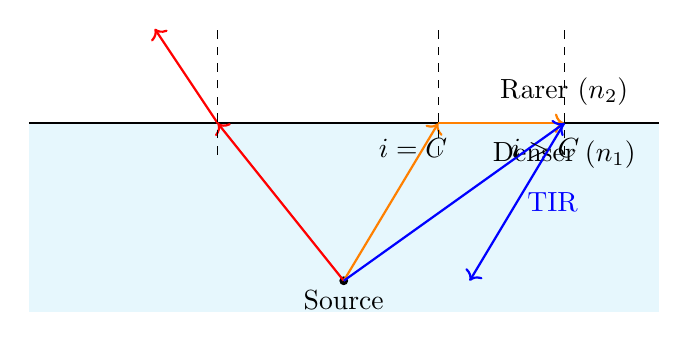
\begin{tikzpicture}[scale=0.8]
    % Mediums
    \fill[cyan!10] (-5,-3) rectangle (5,0);
    \draw[thick] (-5,0) -- (5,0);
    \node at (3.5,-0.5) {Denser ($n_1$)};
    \node at (3.5,0.5) {Rarer ($n_2$)};
    
    % Source
    \coordinate (S) at (0,-2.5);
    \fill (S) circle (2pt) node[below] {Source};
    
    % Ray 1: Refraction (Small angle)
    \draw[red, thick, ->] (S) -- (-2,0);
    \draw[red, thick, ->] (-2,0) -- (-3,1.5);
    \draw[dashed] (-2,-0.5) -- (-2,1.5); % Normal
    
    % Ray 2: Critical Angle (90 degree refraction)
    \draw[orange, thick, ->] (S) -- (1.5,0);
    \draw[orange, thick, ->] (1.5,0) -- (3.5,0);
    \draw[dashed] (1.5,-0.5) -- (1.5,1.5); % Normal
    \node at (1.1, -0.4) {\(i=C\)};
    
    % Ray 3: TIR (i > C)
    \draw[blue, thick, ->] (S) -- (3.5,0);
    \draw[blue, thick, ->] (3.5,0) -- (2,-2.5) node[midway, right] {TIR};
    \draw[dashed] (3.5,-0.5) -- (3.5,1.5); % Normal
    \node at (3.2, -0.4) {\(i>C\)};
    
\end{tikzpicture}
\caption{Total Internal Reflection}
\end{figure}

\paragraph{Conditions for TIR:}
\begin{enumerate}
    \item Light must travel from Denser to Rarer medium.
    \item Angle of incidence must be greater than Critical angle (\(i > C\)).
\end{enumerate}

\paragraph{Mnemonic:} \emph{Denser to Rarer, Angle > Critical = Reflection.}

\noindent \textbf{Question 4(b)} \\
\textbf{Answer the following questions. (Any 2 out of 3)}

\subsection{Question 4(b)(1) [4 marks]}
\textbf{Draw the symbols for (1) p-n junction diode (2) Zener diode and Define: (3) valance electron (4) doping process.}

\subsubsection{Solution}

\paragraph{1. Symbols:}
\begin{figure}[H]
    \centering
    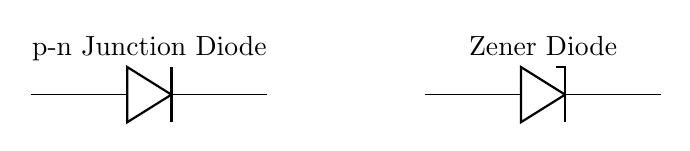
\begin{tikzpicture}
        % PN Junction Diode
        \draw (0,0) to[D, l=p-n Junction Diode] (3,0);
        
        % Zener Diode
        \draw (5,0) to[zD, l=Zener Diode] (8,0);
    \end{tikzpicture}
    \caption{Symbols of p-n Junction Diode and Zener Diode}
\end{figure}

\paragraph{2. Definitions:}

\begin{enumerate}
    \item[(3)] \textbf{Valence Electron:} The electrons present in the \textbf{outermost orbit} (shell) of an atom are called valence electrons. They are loosely bound to the nucleus compared to inner electrons. These electrons are responsible for determining the valency and participating in chemical bonding and electrical conduction in the material.
    \item[(4)] \textbf{Doping Process:} The process of deliberately adding a controlled amount of suitable \textbf{impurity} (called dopant) to a pure intrinsic semiconductor (like Si or Ge) to essentially increase its electrical conductivity is called doping. For example, adding Arsenic creates n-type, while adding Gallium creates p-type semiconductors.
\end{enumerate}

\paragraph{Mnemonic:} \emph{Valence = Outer, Doping = Adding Impurity.}

\subsection{Question 4(b)(2) [4 marks]}
\textbf{Explain construction of optical fiber with figure in detail.}

\subsubsection{Solution}
\paragraph{Construction:} \textbf{Optical Fiber Construction:}
An optical fiber consists of three concentric cylindrical layers:

\begin{enumerate}
    \item \textbf{Core:} The innermost central part made of high-quality glass or plastic. It travels the light signal. It has a high refractive index ($n_1$).
    \item \textbf{Cladding:} The middle layer surrounding the core. It has a slightly \textbf{lower refractive index} ($n_2 < n_1$) than the core. This condition ($n_{core} > n_{cladding}$) causes Total Internal Reflection (TIR), confining light within the core.
    \item \textbf{Buffer Coating (Jacket):} The outermost plastic layer that protects the fiber from moisture, physical damage, and crushing.
\end{enumerate}

\begin{figure}[H]
\centering
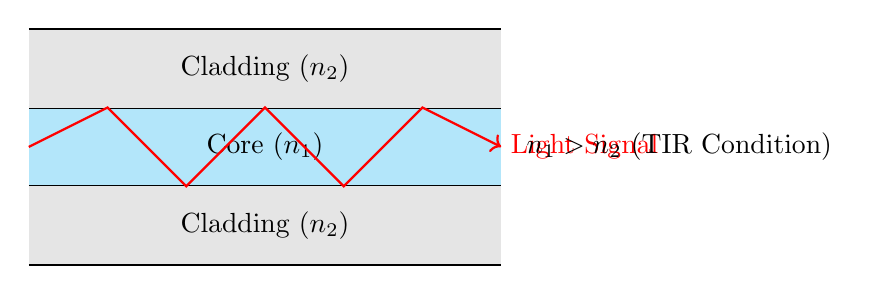
\begin{tikzpicture}
    % Core
    \fill[cyan!30] (0,1) rectangle (6,2);
    \draw[thick] (0,1) -- (6,1);
    \draw[thick] (0,2) -- (6,2);
    \node at (3,1.5) {Core ($n_1$)};
    
    % Cladding
    \fill[gray!20] (0,0) rectangle (6,1);
    \fill[gray!20] (0,2) rectangle (6,3);
    \draw[thick] (0,0) -- (6,0);
    \draw[thick] (0,3) -- (6,3);
    \node at (3,0.5) {Cladding ($n_2$)};
    \node at (3,2.5) {Cladding ($n_2$)};
    
    % Propagating light ray
    \draw[red, thick, ->] (0,1.5) -- (1,2) -- (2,1) -- (3,2) -- (4,1) -- (5,2) -- (6,1.5);
    \node[red, right] at (6,1.5) {Light Signal};

    % Labelling n1 > n2
    \node[right] at (6.2, 1.5) {\(n_1 > n_2\) (TIR Condition)};
\end{tikzpicture}
\caption{Structure of Optical Fiber}
\end{figure}

\paragraph{Mnemonic:} \emph{Core keeps Light (High n), Cladding reflects (Low n), Jacket protects.}

\subsection{Question 4(b)(3) [4 marks]}
\textbf{Explain bridge rectifier with its circuit diagram, input and output waveforms.}

\subsubsection{Solution}
\textbf{Bridge Rectifier:}
A bridge rectifier uses \textbf{four diodes} ($D_1, D_2, D_3, D_4$) arranged in a bridge configuration to convert AC voltage into full-wave pulsating DC voltage.

\paragraph{Working:}
\begin{itemize}
    \item \textbf{Positive Cycle:} Diodes \(D_1\) and \(D_3\) behave as forward biased (conduct), while \(D_2\) and \(D_4\) are reverse biased. Current flows through the load.
    \item \textbf{Negative Cycle:} Diodes \(D_2\) and \(D_4\) conduct, while \(D_1\) and \(D_3\) are reverse biased. Current flows through the load in the \textbf{same direction}.
\end{itemize}

\begin{figure}[H]
\centering
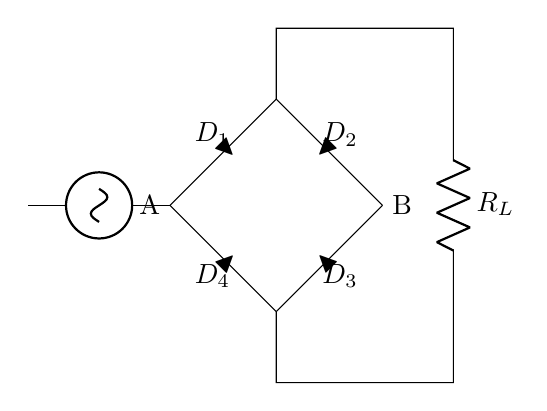
\begin{tikzpicture}[scale=0.9]
    \draw (0,0) node[left] {A} -- (1.5,1.5) coordinate (top);
    \draw (0,0) -- (1.5,-1.5) coordinate (bottom);
    \draw (3,0) node[right] {B} -- (1.5,1.5);
    \draw (3,0) -- (1.5,-1.5);
    
    % Diodes
    \draw (0.8,0.8) node[rotate=-45] {\(\blacktriangleright\)}; % D1ish
    \draw (2.2,0.8) node[rotate=-135] {\(\blacktriangleright\)}; % D2ish
    \draw (0.8,-0.8) node[rotate=45] {\(\blacktriangleright\)}; % D4ish
    \draw (2.2,-0.8) node[rotate=135] {\(\blacktriangleright\)}; % D3ish
    
    % Labels (Simulation)
    \node at (0.6,1) {\(D_1\)};
    \node at (2.4,1) {\(D_2\)};
    \node at (0.6,-1) {\(D_4\)};
    \node at (2.4,-1) {\(D_3\)};
    
    % AC Input
    \draw (-2, 0) to[sinusoidal voltage source] (0,0);
    
    % Load - Taken from Top and Bottom
    \draw (1.5,1.5) -- (1.5, 2.5) -- (4, 2.5) to[R, l=\(R_L\)] (4, -2.5) -- (1.5, -2.5) -- (1.5, -1.5);
    
\end{tikzpicture}
\caption{Bridge Rectifier Circuit}
\end{figure}

\begin{figure}[H]
    \centering
    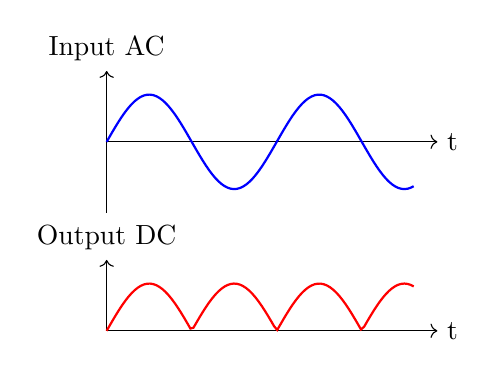
\begin{tikzpicture}[scale=0.6]
        % Input
        \draw[->] (0,0) -- (7,0) node[right] {t};
        \draw[->] (0,-1.5) -- (0,1.5) node[above] {Input AC};
        \draw[blue, thick] plot[domain=0:6.5, samples=100] (\x, {sin(\x*100)});
        
        % Output
        \begin{scope}[yshift=-4cm]
            \draw[->] (0,0) -- (7,0) node[right] {t};
            \draw[->] (0,0) -- (0,1.5) node[above] {Output DC};
            \draw[red, thick] plot[domain=0:6.5, samples=100] (\x, {abs(sin(\x*100))});
        \end{scope}
    \end{tikzpicture}
    \caption{Input and Output Waveforms}
\end{figure}

\paragraph{Mnemonic:} \emph{4 Diodes Bridge, Full Wave Output (All humps positive).}

% ========================================
% QUESTION 5: Short Questions (14 marks)
% Demonstrates: 3 marks and 4 marks questions with Circuit Diagrams and Logic Gates
% ========================================

\section{Question 5}

\noindent \textbf{Question 5(a)} \\
\textbf{Answer the following questions. (Any 2 out of 3)}

\subsection{Question 5(a)(1) [3 marks]}
\textbf{Explain OR, AND and NOT gates.}

\subsubsection{Solution}
\paragraph{Definitions:} \textbf{Logic Gates:}
\begin{enumerate}
    \item \textbf{OR Gate:} It has two or more inputs and one output. The output is HIGH (1) if \textbf{any} of the inputs is HIGH. Boolean Expression: \(Y = A + B\).
    \item \textbf{AND Gate:} It has two or more inputs and one output. The output is HIGH (1) only if \textbf{all} inputs are HIGH. Boolean Expression: \(Y = A \cdot B\).
    \item \textbf{NOT Gate (Inverter):} It has only one input and one output. The output is the inverse of the input. Boolean Expression: \(Y = \bar{A}\).
\end{enumerate}

\begin{figure}[H]
    \centering
    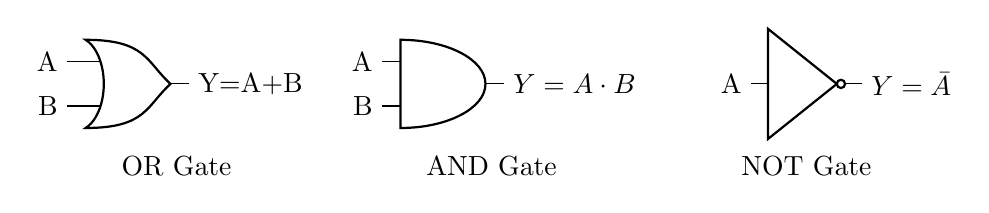
\begin{tikzpicture}
        % OR Gate
        \node[or port] (or) at (0,0) {};
        \node[left] at (or.in 1) {A};
        \node[left] at (or.in 2) {B};
        \node[right] at (or.out) {Y=A+B};
        \node[below] at (0,-0.8) {OR Gate};

        % AND Gate
        \node[and port] (and) at (4,0) {};
        \node[left] at (and.in 1) {A};
        \node[left] at (and.in 2) {B};
        \node[right] at (and.out) {\(Y=A \cdot B\)};
        \node[below] at (4,-0.8) {AND Gate};

        % NOT Gate
        \node[not port] (not) at (8,0) {};
        \node[left] at (not.in) {A};
        \node[right] at (not.out) {\(Y=\bar{A}\)};
        \node[below] at (8,-0.8) {NOT Gate};
    \end{tikzpicture}
    \caption{Logic Gates}
\end{figure}

\paragraph{Mnemonic:} \emph{OR=Any, AND=All, NOT=Inverse.}

\subsection{Question 5(a)(2) [3 marks]}
\textbf{Explain n-type semiconductor.}

\subsubsection{Solution}
\paragraph{Explanation:} \textbf{n-type Semiconductor:}
\begin{itemize}
    \item It is an extrinsic semiconductor obtained by doping a pure intrinsic semiconductor (Group 14, e.g., Silicon, Germanium) with a pentavalent impurity (Group 15, e.g., Phosphorus, Arsenic, Antimony).
    \item The impurity atom has 5 valence electrons. 4 form covalent bonds with 4 neighboring Si atoms, and the \textbf{5th electron remains free}.
    \item Here, electrons are \textbf{majority charge carriers} and holes are minority charge carriers.
    \item It is electrically neutral.
\end{itemize}

\begin{figure}[H]
    \centering
    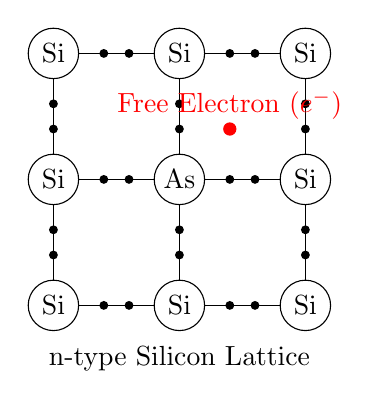
\begin{tikzpicture}[scale=0.8]
        % Atom Grid
        \foreach \x in {0,2,4}
            \foreach \y in {0,2,4} {
                \draw (\x,\y) circle (0.4);
            }
        
        % Labels
        \node at (0,0) {Si}; \node at (2,0) {Si}; \node at (4,0) {Si};
        \node at (0,2) {Si}; \node at (2,2) {As}; \node at (4,2) {Si}; % Center is Impurity
        \node at (0,4) {Si}; \node at (2,4) {Si}; \node at (4,4) {Si};
        
        % Bonds
        \draw (0.4,0) -- (1.6,0); \draw (2.4,0) -- (3.6,0);
        \draw (0.4,2) -- (1.6,2); \draw (2.4,2) -- (3.6,2);
        \draw (0.4,4) -- (1.6,4); \draw (2.4,4) -- (3.6,4);
        
        \draw (0,0.4) -- (0,1.6); \draw (2,0.4) -- (2,1.6); \draw (4,0.4) -- (4,1.6);
        \draw (0,2.4) -- (0,3.6); \draw (2,2.4) -- (2,3.6); \draw (4,2.4) -- (4,3.6);
        
        % Electrons (Dots on bonds)
        \foreach \x in {0.8, 1.2, 2.8, 3.2}
            \foreach \y in {0,2,4} \fill (\x,\y) circle (2pt);
            
        \foreach \x in {0,2,4}
            \foreach \y in {0.8, 1.2, 2.8, 3.2} \fill (\x,\y) circle (2pt);
            
        % Free Electron
        \fill[red] (2.8, 2.8) circle (3pt) node[right, above] {Free Electron ($e^-$)};
        \node[below] at (2, -0.5) {n-type Silicon Lattice};
    \end{tikzpicture}
    \caption{n-type Semiconductor (Pentavalent Doping)}
\end{figure}

\paragraph{Mnemonic:} \emph{n-type = Negative (electron) majority, Pentavalent impurity.}

\subsection{Question 5(a)(3) [3 marks]}
\textbf{Light enters in glass medium from air. Glass has refractive index is 1.56. So find velocity of light in glass. \(C=3 \times 10^8 m/s\).}

\subsubsection{Solution}
\textbf{Given Data:}
\begin{itemize}
    \item Refractive Index of glass (\(n\)) = 1.56
    \item Speed of light in vacuum (\(c\)) = \(3 \times 10^8 \, m/s\)
\end{itemize}

\textbf{Formula:}
The refractive index (\(n\)) is defined as the ratio of speed of light in vacuum (\(c\)) to the speed of light in the medium (\(v\)).
\[ n = \frac{c}{v} \]

\textbf{Calculation:}
Rearranging to solve for velocity in glass:
\[ v = \frac{c}{n} \]
Substituting the values:
\[ v = \frac{3 \times 10^8}{1.56} \]

\[ v \approx 1.923 \times 10^8 \, m/s \]
This indicates that light travels about 1.56 times slower in glass than in vacuum.

\paragraph{Answer:} The velocity of light in glass is approximately \(\mathbf{1.92 \times 10^8 \, m/s}\).

\paragraph{Conclusion:}
The refractive index is physically a ratio of speeds and is always greater than 1. This confirms that light travels slower in a denser medium like glass compared to vacuum. The higher the refractive index, the lower the velocity in that medium.




\paragraph{Mnemonic:} \emph{v = c / n (Velocity decreases in denser medium).}

\noindent \textbf{Question 5(b)} \\
\textbf{Answer the following questions. (Any 2 out of 3)}

\subsection{Question 5(b)(1) [4 marks]}
\textbf{Explain forward bias characteristics of p-n junction diode.}

\subsubsection{Solution}
\textbf{Forward Bias Characteristics:}
\begin{itemize}
    \item When the \textbf{p-type region} is connected to the \textbf{positive terminal} and the \textbf{n-type region} to the \textbf{negative terminal} of a battery, the diode is said to be forward biased.
    \paragraph{Explanation:}
    \item \textbf{Si and Ge are semiconductors:} Silicon (Si) and Germanium (Ge) are semiconductor materials.
    \item \textbf{Potential Barrier:} The minimum voltage required to cross the depletion layer in a p-n junction. \(0.7V\) for Si, \(0.3V\) for Ge. This depends on the energy band gap.
    \item The depletion width \textbf{decreases} and the potential barrier is lowered, allowing majority carriers to cross the junction easily.
    \item A large current flows in the milli-ampere (\(mA\)) range.
    \item The current increases exponentially with voltage after overcoming the threshold voltage (\(0.7V\) for Si, \(0.3V\) for Ge), known as \textbf{Knee Voltage}.
\end{itemize}

\begin{figure}[H]
    \centering
    \begin{tikzpicture}[scale=0.8]
        % Circuit
        \draw (0,0) to[D, l=Diode] (3,0);
        \draw (3,0) -- (3,-2) -- (0,-2) to[battery1, l=Battery] (0,0);
        \node at (1.5, -2.5) {Forward Bias Connection};
        
        % Graph
        \begin{scope}[xshift=5cm, yshift=-1.5cm]
            \draw[->] (0,0) -- (3,0) node[right] {\(V_F\) (Volts)};
            \draw[->] (0,0) -- (0,3) node[above] {\(I_F\) (mA)};
            \draw[blue, thick] plot[domain=0:2.5, samples=100] (\x, {0.1*exp(2*\x)-0.1});
            \node at (2,2) {Exponential Rise};
            \node at (1.5,-0.5) {VI Characteristic};
        \end{scope}
    \end{tikzpicture}
    \caption{Forward Bias Circuit and V-I Characteristics}
\end{figure}

\paragraph{Mnemonic:} \emph{Forward = P to Plus, Current Flows, Barrier Lowers.}

\subsection{Question 5(b)(2) [4 marks]}
\textbf{Explain working of Zener diode as a voltage regulator.}

\subsubsection{Solution}
\paragraph{Working:} \textbf{Zener Diode as Voltage Regulator:}

\begin{itemize}
    \item A Zener diode is designed to operate in the \textbf{reverse breakdown region}.
    \item In this region, the voltage across the Zener diode ($V_Z$) remains \textbf{constant} even if the current through it ($I_Z$) varies significantly.
    \item It is connected in \textbf{parallel} with the load resistance ($R_L$) and in reverse bias.
    \item A series resistor ($R_S$) creates a voltage drop to absorb fluctuations in input voltage ($V_{in}$).
    \item If \(V_{in}\) increases, current through Zener increases, voltage drop across \(R_S\) increases, but voltage across load (\(V_Z\)) remains constant.
\end{itemize}

\begin{figure}[H]
    \centering
    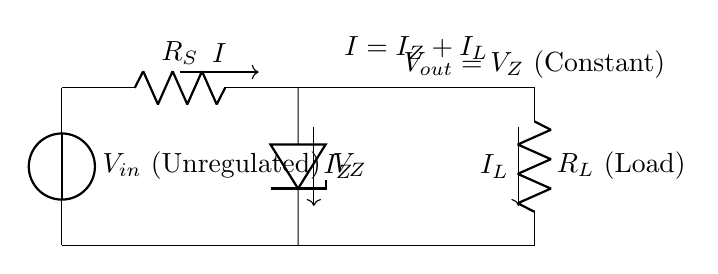
\begin{tikzpicture}
        \draw (0,2) to[V, l=\(V_{in}\) (Unregulated)] (0,0);
        \draw (0,2) to[R, l=\(R_S\)] (3,2);
        \draw (3,2) to[zD, l=\(V_Z\)] (3,0);
        \draw (3,2) -- (6,2) to[R, l=\(R_L\) (Load)] (6,0) -- (0,0);
        
        \node at (6,2.3) {\(V_{out} = V_Z\) (Constant)};
        \draw[->] (1.5, 2.2) -- (2.5, 2.2) node[midway, above] {\(I\)};
        \draw[->] (3.2, 1.5) -- (3.2, 0.5) node[midway, right] {\(I_Z\)};
        \draw[->] (5.8, 1.5) -- (5.8, 0.5) node[midway, left] {\(I_L\)};
        \node at (4.5, 2.5) {\(I = I_Z + I_L\)};
    \end{tikzpicture}
    \caption{Zener Diode Voltage Regulator Circuit}
\end{figure}

\paragraph{Mnemonic:} \emph{Zener in Reverse Parallel, Constant Voltage.}

\subsection{Question 5(b)(3) [4 marks]}
\textbf{An optical fiber has value of refractive indices for core and cladding are 1.48 and 1.45, respectively. Calculate numerical aperture and acceptance angle of optical fiber.}

\subsubsection{Solution}
\textbf{Given Data:}
\begin{itemize}
    \item Refractive index of core ($n_1$) = 1.48
    \item Refractive index of cladding ($n_2$) = 1.45
\end{itemize}

\textbf{Formulas:}
\begin{enumerate}
    \item \textbf{Numerical Aperture (NA):}
    \[ NA = \sqrt{n_1^2 - n_2^2} \]
    \item \textbf{Acceptance Angle (\(\theta_a\)):}
    \[ \theta_a = \sin^{-1}(NA) \]
\end{enumerate}

\textbf{Calculations:}
\textbf{1. Numerical Aperture (NA):}
This represents the light gathering ability of the fiber.
\[ NA = \sqrt{(1.48)^2 - (1.45)^2} \]
\[ NA = \sqrt{2.1904 - 2.1025} \]
\[ NA = \sqrt{0.0879} \]
\[ NA \approx 0.2965 \]

\textbf{2. Acceptance Angle (\(\theta_a\)):}
The maximum angle of incidence at which light is accepted into the core.
\[ \theta_a = \sin^{-1}(NA) \]
\[ \theta_a = \sin^{-1}(0.2965) \]
\[ \theta_a \approx 17.25^\circ \]

\paragraph{Answer:}
\begin{itemize}
    \item Numerical Aperture (NA) = \textbf{0.2965}
    \item Acceptance Angle (\(\theta_a\)) = \(\mathbf{17.25^\circ}\)
\end{itemize}

\paragraph{Significance:}
The Numerical Aperture (NA) value of 0.2965 indicates the fiber's ability to accept light. A higher NA would allow the fiber to accept light from a wider cone, coupling more power from the source. The acceptance angle of approximately \(17^\circ\) defines the ``cone of acceptance'' within which light rays must enter to undergo Total Internal Reflection and propagate through the core. This fiber is suitable for short-distance, low-power communication. For long-distance communication, single-mode fibers with lower NA and smaller acceptance angles are typically used to minimize dispersion.

\paragraph{Mnemonic:} \emph{NA = Root(n1 sq - n2 sq).}

\end{document}




